\chapter{Introduction}

\section{Project summary}
k

\subsection{Motivation}
k

\subsection{The system}
k

\section{System description}
\begin{figure}[H]
	\centering
	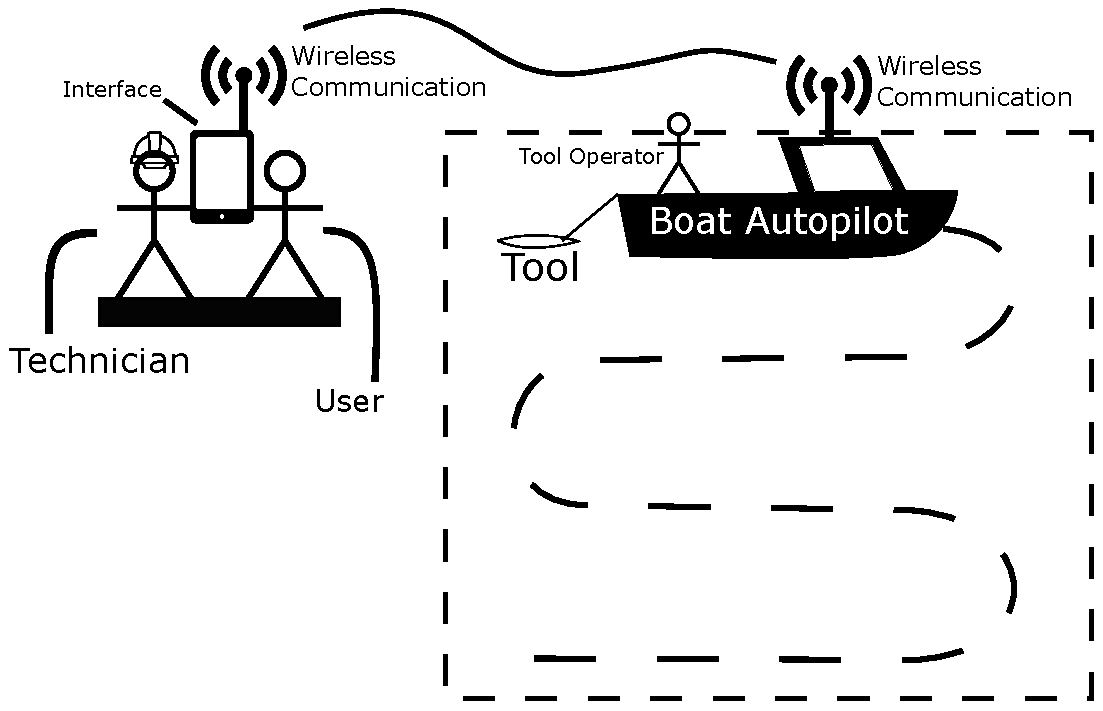
\includegraphics[width=1\linewidth]{Images/rich_image}
	\caption{Rich image}
\end{figure}

\begin{figure}[H]
	\centering
	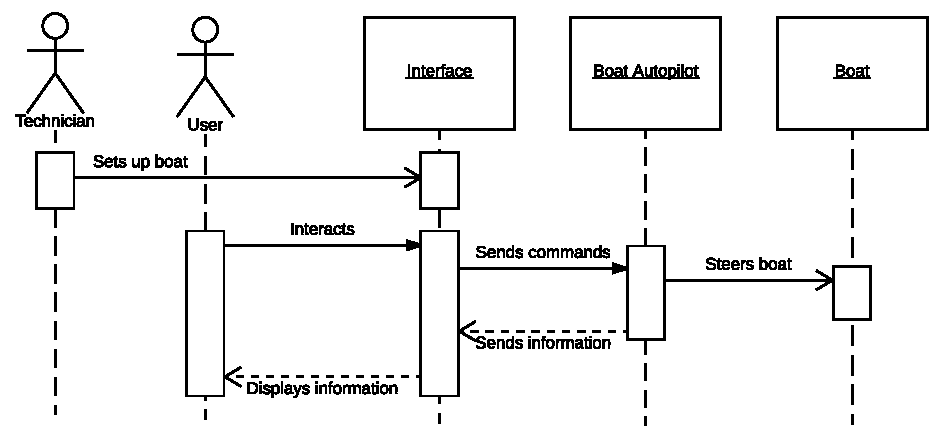
\includegraphics[width=1\linewidth]{Images/General_SD}
	\caption{General sequence diagram}
\end{figure}

\section{System considerations}
k

\subsection{Drivetrain}

k

\subsection{Steering}
k

\subsection{Communications}
k

THIS IS FROM THE PRE-PROJECT, USE IT TO WRITE THESE

The problem description is taken from the project offer on blackboard\cite{EIVA-description}

The market for unmanned surface vessels (sailing drones) is growing, and there is a need for an open architecture auto-pilot that is usable on different platforms.

This project is about designing and implementing the electronics and embedded software for an autopilot which is able to receive steering commands from a navigation system (distance to go left/right) and from thoes instructions, steer a small boat (et. control left/right thrusters).


\paragraph{Project details}
\begin{itemize}
\item PCB design of autopilot electronics (if something existing cannot be used)
\item Implement PID control loop to get back on course based on received left/right commands
\item Control of thrusters in case of two-thruster catamaran
\item Control of wheel in case of outboard motor on boat
%Should this be here?
\item Test trials at sea
\item EIVA will provide necessary hardware, include test boats / catamarans, including PCB production cost
\item EIVA will provide work-space (desk, lunch etc) at EIVA's facilities
\item IF the project is successful, EIVA will offer to finalise the product and make it available for sale with a commision to the student
\end{itemize}